\documentclass[11pt]{article}

\usepackage[a4paper,margin=1in]{geometry}
\usepackage[T1]{fontenc}
\usepackage[utf8]{inputenc}
\usepackage{lmodern}
\usepackage{microtype}
\usepackage{amsmath,amssymb,amsthm,mathtools}
\usepackage{booktabs}
\usepackage{graphicx}
\usepackage{float}
\usepackage{placeins}
\usepackage{enumitem}
\usepackage[numbers,sort&compress]{natbib}
\usepackage{xcolor}
\usepackage{xurl}
\usepackage[colorlinks=true,linkcolor=blue!55!black,citecolor=blue!55!black,urlcolor=blue!55!black]{hyperref}
\usepackage[nameinlink,noabbrev]{cleveref}

\setlength{\parindent}{1.4em}
\setlength{\parskip}{0.15em}
\setlist{itemsep=0.25em,topsep=0.35em}

\newtheorem{theorem}{Theorem}[section]
\newtheorem{proposition}[theorem]{Proposition}
\newtheorem{lemma}[theorem]{Lemma}
\newtheorem{corollary}[theorem]{Corollary}
\theoremstyle{definition}
\newtheorem{definition}[theorem]{Definition}
\theoremstyle{remark}
\newtheorem{remark}[theorem]{Remark}

\newcommand{\R}{\mathbb R}
\newcommand{\C}{\mathbb C}
\newcommand{\uc}{u_{\mathrm c}}
\newcommand{\cK}{\mathcal K}
\newcommand{\cP}{\mathcal P}
\newcommand{\cT}{\mathcal T}
\newcommand{\Id}{\mathrm I}
\newcommand{\erfop}{\operatorname{erf}}
\newcommand{\erfcop}{\operatorname{erfc}}

\title{\textbf{Square-Root Parity Splitting}\\
\textbf{at a Quadratic Band-Merging Map:}\\[0.35em]
\large Coupled Critical-Value Boundary Layers and a Corrected Small-Noise Law}
\author{Liang Wang\\
\small School of Artificial Intelligence and Automation,\\[-0.2em]
\small Huazhong University of Science and Technology, Wuhan 430074, P.R. China\\
\small \texttt{wangliang.f@gmail.com}}
\date{July 2026}

\begin{document}

\maketitle

\begin{abstract}
At the algebraic band-merging parameter of $f_u(x)=1-u x^2$, deterministic
dynamics has two cyclic components and the zero-noise Markov operator has a
parity eigenvalue $-1$.  Positive Gaussian noise makes the operator strongly
mixing and moves this mode to a simple real resonance
$\lambda_-(\sigma)>-1$.  Previous dense computations on
$0.01\le\sigma\le0.03$ gave the striking fit
$1+\lambda_-(\sigma)\asymp\sigma^{2/3}$.  We show that this is a crossover,
not the small-noise exponent.

Two boundary layers determine the actual splitting.  At the repelling
component boundary $r=u_{\mathrm c}-1$, the rescaled left parity observable
is exactly
\[
 H(\xi)=-\erfop(\kappa\xi),
 \qquad
 \kappa=\sqrt{\frac{\lambda^2-1}{2}},
 \qquad
 \lambda=2u_{\mathrm c}r.
\]
It solves the Gaussian dilation equation
$\mathbb E H(-\lambda\xi+Z)=-H(\xi)$.  A second layer is created at the
critical value $1$.  If $\rho_c$ is the central-component invariant density
at the critical point, then the signed right eigenmeasure satisfies
\[
 -\sqrt\sigma\,g_{\sigma,-}(1-\sigma\xi)\longrightarrow
 R(\xi)
 =\rho_c\int_0^\infty
 \frac{\phi(u_{\mathrm c}q^2-\xi)}{\Phi(u_{\mathrm c}q^2)}\,dq.
\]
Pairing the two layers gives the nonanalytic spectral law
\[
 \boxed{
  1+\lambda_-(\sigma)=C_*\sqrt\sigma+o(\sqrt\sigma)},
 \qquad
 C_*=\int_0^\infty R(\xi)\erfcop(a\xi)\,d\xi>0,
\]
where $a=2u_{\mathrm c}\kappa/\lambda$.  The exact integral evaluates
numerically to
\[
 \rho_c=0.562641254486572\ldots,
 \qquad
 C_*=0.105258535936908\ldots.
\]
Consequently the parity lifetime is asymptotic to
$(C_*\sqrt\sigma)^{-1}$, and the $2/3$-scaled gap diverges like
$C_*\sigma^{-1/6}$.

Sparse folded computations with up to $204800$ states reach
$\sigma=10^{-4}$.  They reproduce the old-window exponent $0.667416$, but
the local exponent falls to $0.51613$ and
$(1+\lambda_-)/\sqrt\sigma$ moves toward the predicted constant.  These
computations audit the asymptotic mechanism; the square-root law follows from
the spectral-stability and boundary-layer argument.
\end{abstract}

\noindent\textbf{Keywords:} random perturbation; transfer operator; parity
resonance; boundary layer; quadratic map; metastable spectrum; critical
value; nonanalytic eigenvalue splitting.

\medskip
\noindent\textbf{MSC 2020:} 37E05; 37D25; 47A55; 60J05; 65P30.

\section{Introduction}
\label{sec:introduction}

Noise destroys exact cyclic decompositions.  The subtle question is how
quickly.  At a quadratic band-merging parameter, the deterministic attractor
has two components exchanged by one iterate.  The associated Markov operator
therefore has peripheral eigenvalues $1$ and $-1$.  Every positive Gaussian
noise makes the transition kernel strictly positive, leaving only the Perron
root on the unit circle.  The former parity mode becomes a long-lived negative
resonance.

The preceding long-cycle study isolated this resonance and found
\begin{equation}\label{eq:old-fit}
 1+\lambda_-(\sigma)simeq
 0.2881505\,\sigma^{0.6674161}
\end{equation}
over its five smallest noise levels
$0.01\le\sigma\le0.03$ \citep{WangLongCycle2026}.  It explicitly kept the
$2/3$ exponent outside the theorem layer.  Subsequent work completed the
deterministic side: an analytic circle lift exposed the postcritical factors,
and validated Wiener--Taylor bounds proved their noncancellation
\citep{WangPostcritical2026,WangValidatedGap2026}.  Thus the stochastic
splitting in \eqref{eq:old-fit} is now the remaining parity question.

The main point of this paper is that a single local layer gives the wrong
answer.  Smoothing the component jump at the repelling fixed point produces
an exact error-function profile, but that profile is locally balanced and
does not split the eigenvalue at leading order.  Splitting occurs one
preimage farther away, at the endpoint $x=1$ that maps exactly onto the
component boundary.  The invariant density there is itself a noise-rounded
square-root spike created by the critical point.  Its height is
$\sigma^{-1/2}$ and its width is $\sigma$; their product forces the
$\sqrt\sigma$ law.

\subsection*{Main results and status}

\begin{enumerate}[label=\textbf{R\arabic*.},leftmargin=3.2em]
 \item Standard stochastic spectral stability for the postcritically finite
 quadratic map gives a unique simple real resonance
 $\lambda_-(\sigma)\to-1$.

 \item The component-boundary observable has the exact universal profile
 $H(\xi)=-\erfop(\kappa\xi)$.  No fitted parameter enters $\kappa$.

 \item The critical point and the truncation normalizer produce a second,
 explicit endpoint-density profile $R$.  The factor
 $\Phi(u_{\mathrm c}q^2)^{-1}$ in $R$ is essential; dropping row
 normalization changes the leading constant.

 \item A solvability pairing between the left profile $H$ and the signed
 right density $R$ proves
 \[
  1+\lambda_-(\sigma)=C_*\sqrt\sigma+o(\sqrt\sigma),
  \qquad C_*>0.
 \]

 \item Hence the parity e-folding time is
 $(C_*\sqrt\sigma)^{-1}(1+o(1))$.  For
 $m\sqrt\sigma\to t$, the peripheral mode has the crossover
 $(-1)^m e^{-C_*t}$.

 \item The former $2/3$ law is ruled out asymptotically:
 $(1+\lambda_-)/\sigma^{2/3}\to\infty$.  Its accurate appearance on the old
 window is reproduced exactly and explained as preasymptotic drift.

 \item All finite matrices, fitted exponents, and profile comparisons are
 diagnostics.  The decimal evaluation of $C_*$ is numerical, while its
 positive integral formula and the exponent $1/2$ are analytic conclusions.
\end{enumerate}

\section{The folded Gaussian operator and deterministic parity}
\label{sec:operator}

Let $u=\uc$ be the real root in $(1,2)$ of
\begin{equation}\label{eq:cubic}
 u^3-2u^2+2u-2=0,
\end{equation}
and put
\begin{equation}\label{eq:constants}
 r=\uc-1,
 \qquad
 \lambda=2\uc r.
\end{equation}
Then
\begin{equation}\label{eq:critical-orbit}
 0\longmapsto1\longmapsto-r\longmapsto r\longmapsto r,
\end{equation}
and
\begin{equation}\label{eq:numerical-constants}
 \uc=1.543689012692076\ldots,
 \quad
 r=0.543689012692076\ldots,
 \quad
 \lambda=1.678573510428322\ldots.
\end{equation}

Write $f=f_{\uc}$ and fold the signed state by $x\mapsto|x|$.  On $[0,1]$
the deterministic map is
\begin{equation}\label{eq:folded-map}
 T(x)=|1-\uc x^2|.
\end{equation}
Up to the common endpoint $r$, the intervals
\begin{equation}\label{eq:components}
 B=[0,r],
 \qquad
 C=[r,1]
\end{equation}
are exchanged by $T$.  Thus
\begin{equation}\label{eq:hard-parity}
 h_0=\mathbf1_B-\mathbf1_C,
 \qquad
 h_0\circ T=-h_0
\end{equation}
away from the two boundary preimages.

Let
\begin{equation}\label{eq:gaussian}
 \phi_\sigma(t)=\frac1{\sqrt{2\pi}\sigma}
 e^{-t^2/(2\sigma^2)},
 \qquad
 Z_\sigma(x)=\int_{-1}^1\phi_\sigma(y-f(x))\,dy.
\end{equation}
The normalized folded Markov operator acting on observables is
\begin{equation}\label{eq:markov-operator}
 (\cK_\sigma h)(x)
 =\frac1{Z_\sigma(x)}
 \int_{-1}^1\phi_\sigma(y-f(x))h(|y|)\,dy.
\end{equation}
It is compact and strongly positive for every $\sigma>0$.  Its dual density
operator is denoted by $\cP_\sigma$.

\subsection{Peripheral spectral stability}

The map is postcritically finite and Misiurewicz.  Its deterministic transfer
operator is quasi-compact on the standard tower/spike space $\mathcal B$: a
regular bounded-variation part is augmented by the finitely generated
one-sided square-root singularities along \eqref{eq:critical-orbit}
\citep{Misiurewicz1981,KellerNowicki1992,Baladi2000}.  We use $L^1$ as the
weak norm.  The two mixing components give two simple peripheral eigenvalues
$1$ and $-1$.

For completeness, we check the only feature of the present perturbation that
is not covered verbatim by the usual additive-noise construction.  Before
folding, choose a slightly larger ambient interval $J\supset[-1,1]$ with
$f(J)\subset\operatorname{int}J$; the ordinary tower estimates are applied
there.  Let $Q_\sigma$ denote Gaussian convolution after extension by zero,
and put $M_\sigma g=Z_\sigma^{-1}g$.  Restriction and conditioning on the
physical state interval then have the exact factorization
\begin{equation}\label{eq:conditioned-factorization}
 \cP_\sigma g
 =\mathbf1_{[-1,1]}Q_\sigma\cP_0(M_\sigma g).
\end{equation}
On a fixed neighborhood of the critical point,
\begin{equation}\label{eq:normalizer-local}
 Z_\sigma(x)
 =\Phi\!\left(\frac{\uc x^2}{\sigma}\right)
  +O(e^{-c/\sigma^2}).
\end{equation}
Here $\Phi$ is the standard normal distribution function.
Consequently $1\le M_\sigma\le2+o(1)$,
$\operatorname{var}M_\sigma=O(1)$, and, because the regular part of
$\mathcal B$ is bounded near $x=0$,
\begin{equation}\label{eq:normalizer-weak-bound}
 \|(M_\sigma-\Id)g\|_{L^1}
 \le C\sqrt\sigma\,\|g\|_{\mathcal B},
 \qquad
 \|M_\sigma g\|_{\mathcal B}
 \le C\|g\|_{\mathcal B}.
\end{equation}
Indeed, outside $|x|=O(\sqrt\sigma)$ the first difference has a Gaussian
tail in $x^2/\sigma$.  The tower proof of the uniform Lasota--Yorke estimate
uses only critical nonrecurrence and derivative growth; topological mixing is
used later only to remove nontrivial peripheral roots
\citep{BaladiViana1996}.  Inserting \eqref{eq:normalizer-weak-bound} leaves
that proof unchanged.  The compact-support estimates extend to the Gaussian
kernel by applying their variation bounds on dyadic tail shells and summing
the exponentially decaying shell masses.  Thus, for some $A,B<\infty$
and $\vartheta<1$, uniformly for small $\sigma$,
\begin{equation}\label{eq:strong-weak-estimates}
 \|\cP_\sigma^n g\|_{\mathcal B}
 \le A\vartheta^n\|g\|_{\mathcal B}+B\|g\|_{L^1},
 \qquad
 \|\cP_\sigma-\cP_0\|_{\mathcal B\to L^1}=o(1).
\end{equation}
These are precisely the strong/weak hypotheses of the Keller--Liverani
theorem \citep{KellerLiverani1999}.  Notice that the order-one limit of
$M_\sigma$ at $x=0$ is weakly small but cannot be discarded in the boundary
layer calculation below.

\begin{proposition}[Stable negative peripheral resonance]
\label{prop:spectral-stability}
There exist $\sigma_0>0$ and $\epsilon>0$ such that, for
$0<\sigma<\sigma_0$, the spectrum of $\cK_\sigma$ in
$|z+1|<\epsilon$ consists of one simple real eigenvalue
$\lambda_-(\sigma)$.  Moreover
\begin{equation}\label{eq:lambda-convergence}
 \lambda_-(\sigma)\longrightarrow-1.
\end{equation}
There is a real signed eigenmeasure
$g_\sigma(x)\,dx$ of $\cP_\sigma$, normalized as below, which converges in
$L^1$ to the deterministic signed component density and locally uniformly
away from the postcritical set.
\end{proposition}

\begin{proof}
On the tower/spike space, $-1$ is isolated and simple because the square map is
mixing on each component.  The analytic circle realization and its validated
reduced-sector gap provide, for this parameter, an explicit isolation of the
component spectrum \citep{WangValidatedGap2026}.  The uniform
Lasota--Yorke inequality and weak convergence in
\eqref{eq:strong-weak-estimates}, together with the compact strong-to-weak
embedding, give stability of its rank-one spectral projector.  A simple
eigenvalue of a real operator remains real as long as it remains isolated:
otherwise its complex conjugate would be a second eigenvalue in the same
disk.  Applying the convergent projector to $g_0$ and fixing the pairing
normalization below gives $g_\sigma\to g_0$ in $L^1$.  On compact sets
avoiding the finite postcritical set, all relevant inverse branches have
derivative bounded away from zero.  The local transfer equation then upgrades
the regular part to uniform convergence; in particular, for some $\delta>0$,
\begin{equation}\label{eq:central-uniform-convergence}
 \sup_{0\le x\le\delta}|g_\sigma(x)-\rho_D(x)|\longrightarrow0.
\end{equation}
\end{proof}

Near a postcritical spike, the same tower bound gives, after reducing
$\delta$ if necessary,
\begin{equation}\label{eq:spike-majorant}
 |g_\sigma(r+\sigma\xi)|
 \le C\sigma^{-1/2}(1+|\xi|)^{-1/2},
 \qquad |\xi|\le\delta/\sigma.
\end{equation}
This estimate and \eqref{eq:central-uniform-convergence} are the two local
consequences used below.

\section{The deterministic central density}
\label{sec:density}

Let
\begin{equation}\label{eq:central-square}
 S=f^2|_{[-r,r]}.
\end{equation}
This is a mixing full-branch map on the central component.  Its cosine lift
$\pi(\theta)=-r\cos\theta$ is an analytic expanding circle map.  Let
$v(x)$ be the even analytic invariant density in interval coordinates,
normalized by
\begin{equation}\label{eq:v-normalization}
 \frac1{2\pi}\int_0^{2\pi}v(-r\cos\theta)\,d\theta=1.
\end{equation}
The exact Wiener--Taylor construction of the preceding two papers gives
$\cT_1v=v$ and proves that this Perron eigenvalue is simple
\citep{WangPostcritical2026,WangValidatedGap2026}.

Pushing normalized circle measure through the two-sheeted cover gives the
central-component probability density
\begin{equation}\label{eq:rho-D}
 \rho_D(x)=\frac{v(x)}{\pi\sqrt{r^2-x^2}},
 \qquad -r<x<r.
\end{equation}
It is even, integrates to one, is analytic at the critical point $x=0$, and
has the expected square-root endpoint spikes.  Define
\begin{equation}\label{eq:rho-c}
 \rho_c:=\rho_D(0)=\frac{v(0)}{\pi r}>0.
\end{equation}

The Taylor implementation solves the normalized Perron equation at degrees
$80,120,160$ and obtains the identical displayed values
\begin{equation}\label{eq:rho-c-numerical}
 v(0)=0.961019061704572\ldots,
 \qquad
 \rho_c=0.562641254486572\ldots.
\end{equation}
These decimals are used only to evaluate the final integral; the theorem uses
the exact quantity in \eqref{eq:rho-c}.

For later normalization, the zero-noise signed parity density on the folded
space is
\begin{equation}\label{eq:signed-zero-density}
 g_0(x)=
 \begin{cases}
  \rho_D(x),&x\in B,\\
  -\frac12\rho_C(x),&x\in C,
 \end{cases}
\end{equation}
where $\rho_C=f_*\rho_D$ is the normalized density on the outer component.
Evenness of $\rho_D$ and normalization of $\rho_C$ give
\begin{equation}\label{eq:folded-masses}
 \int_0^r\rho_D(x)\,dx=\frac12,
 \qquad
 \int_r^1\rho_C(x)\,dx=1.
\end{equation}
Thus both pieces in \eqref{eq:signed-zero-density} have total absolute mass
$1/2$, and
\begin{equation}\label{eq:pair-normalization}
 \int_0^1h_0(x)g_0(x)\,dx=1.
\end{equation}
We normalize $g_\sigma$ by continuation of
\eqref{eq:pair-normalization}.

\section{The repelling-boundary eigenprofile}
\label{sec:left-layer}

Let $Z$ be standard normal and define
\begin{equation}\label{eq:kappa-H}
 \kappa=\sqrt{\frac{\lambda^2-1}{2}},
 \qquad
 H(\xi)=-\erfop(\kappa\xi).
\end{equation}
Then $H(-\infty)=1$, $H(+\infty)=-1$, so it smooths the hard parity jump in
the correct orientation.

\begin{lemma}[Exact Gaussian dilation profile]
\label{lem:exact-profile}
For every $\xi\in\R$,
\begin{equation}\label{eq:dilation-equation}
 \mathbb E\,H(-\lambda\xi+Z)=-H(\xi).
\end{equation}
\end{lemma}

\begin{proof}
The elementary Gaussian identity
\begin{equation}\label{eq:erf-identity}
 \mathbb E\,\erfop(A+BZ)
 =\erfop\!\left(\frac{A}{\sqrt{1+2B^2}}\right)
\end{equation}
follows by differentiating both sides in $A$ and matching the value at zero.
Since $1+2\kappa^2=\lambda^2$, substituting
$A=-\kappa\lambda\xi$ and $B=\kappa$ proves
\eqref{eq:dilation-equation}.
\end{proof}

Use the global approximate parity observable
\begin{equation}\label{eq:h-sigma}
 \widehat h_\sigma(x)=H\!\left(\frac{x-r}{\sigma}\right).
\end{equation}
Near $r$, write $x=r+\sigma\xi$.  Since
\begin{equation}\label{eq:f-at-r}
 f(r+\sigma\xi)=r-\lambda\sigma\xi-\uc\sigma^2\xi^2,
\end{equation}
the full-Gaussian leading part of
$\cK_\sigma\widehat h_\sigma$ is exactly the left side of
\eqref{eq:dilation-equation}.  The row normalizer tends to one exponentially
fast because $r$ is an interior target.  Hence the apparent $O(1)$ smoothing
at $r$ is locally balanced and contributes no leading eigenvalue defect.

The other preimage of the component boundary is the endpoint $x=1$.  Put
$x=1-\sigma\xi$, $\xi\ge0$.  Then
\begin{equation}\label{eq:f-at-one}
 f(1-\sigma\xi)
 =-r+2\uc\sigma\xi+O(\sigma^2\xi^2).
\end{equation}
After folding, the target boundary coordinate is
$-2\uc\xi-Z+o(1)$.  Applying \cref{lem:exact-profile} gives a second exact
Gaussian identity.

\begin{lemma}[Endpoint solvability defect]
\label{lem:endpoint-defect}
Let
\begin{equation}\label{eq:a-definition}
 a=\frac{2\uc\kappa}{\lambda}.
\end{equation}
For every fixed $\xi\ge0$,
\begin{equation}\label{eq:endpoint-defect}
 (\cK_\sigma\widehat h_\sigma+\widehat h_\sigma)
 (1-\sigma\xi)
 \longrightarrow-\erfcop(a\xi).
\end{equation}
If $D_\sigma=\cK_\sigma\widehat h_\sigma+\widehat h_\sigma$, there are
$\delta,C,c>0$ such that
\begin{align}
 |D_\sigma(r+\sigma\xi)|
 &\le C\sigma(1+\xi^2)e^{-c\xi^2}+Ce^{-c/\sigma^2},
 && |\xi|\le\delta/\sigma,
 \label{eq:r-defect-majorant}\\
 |D_\sigma(1-\sigma\xi)|
 &\le Ce^{-c\xi^2}+Ce^{-c/\sigma^2},
 && 0\le\xi\le\delta/\sigma.
 \label{eq:one-defect-majorant}
\end{align}
Outside these two fixed $\delta$-neighborhoods, $D_\sigma=O(e^{-c/\sigma^2})$.
\end{lemma}

\begin{proof}
By \eqref{eq:f-at-one},
\[
 (\cK_\sigma\widehat h_\sigma)(1-\sigma\xi)
 \longrightarrow
 \mathbb E H(-2\uc\xi-Z)
 =\erfop\!\left(\frac{2\uc\kappa}{\lambda}\xi\right).
\]
Meanwhile $\widehat h_\sigma(1-\sigma\xi)\to-1$.  Their sum is
$-\erfcop(a\xi)$.  The remaining estimates follow from Gaussian tails and
the Taylor remainders in \eqref{eq:f-at-r} and \eqref{eq:f-at-one}.  More
explicitly, convolution with $H'$ turns the quadratic displacement
$\uc\sigma\xi^2$ in the rescaled $r$-coordinate into the first bound in
\eqref{eq:r-defect-majorant}; the convolved derivative has Gaussian decay in
$\xi$.  At the endpoint and on the complement, the distance of the image
from the parity boundary gives \eqref{eq:one-defect-majorant} and the stated
off-layer estimate.
\end{proof}

Numerically,
\begin{equation}\label{eq:profile-constants}
 \kappa=0.953312391063827\ldots,
 \qquad
 a=1.753414854465239\ldots.
\end{equation}

\section{The critical-value endpoint density}
\label{sec:right-layer}

The defect in \cref{lem:endpoint-defect} must be paired with the signed right
eigenmeasure near $x=1$.  That density cannot be replaced by its formal
zero-noise spike at the scale $1-x=O(\sigma)$, because the critical source and
the truncation normalizer are resolved on exactly the same scale.

Let $\phi(t)=(2\pi)^{-1/2}e^{-t^2/2}$ and let $\Phi$ be its distribution
function.  Set
\begin{equation}\label{eq:R-profile}
 R(\xi)=\rho_c\int_0^\infty
 \frac{\phi(\uc q^2-\xi)}{\Phi(\uc q^2)}\,dq,
 \qquad \xi\ge0.
\end{equation}

\begin{lemma}[Critical endpoint layer]
\label{lem:endpoint-density}
For each compact interval of $\xi\ge0$,
\begin{equation}\label{eq:endpoint-density-limit}
 -\sqrt\sigma\,g_\sigma(1-\sigma\xi)
 \longrightarrow R(\xi)
\end{equation}
locally uniformly.  Moreover there is an integrable majorant after
multiplication by the endpoint defect: for some $\delta,C>0$,
\begin{equation}\label{eq:endpoint-density-majorant}
 \sqrt\sigma\,|g_\sigma(1-\sigma\xi)|
 \le C(1+\xi)^{-1/2},
 \qquad 0\le\xi\le\delta/\sigma.
\end{equation}
In addition,
\begin{equation}\label{eq:R-tail}
 R(\xi)\sim\frac{\rho_c}{2\sqrt{\uc\xi}}
 \qquad(\xi\to\infty).
\end{equation}
\end{lemma}

\begin{proof}
The only deterministic sources that can reach $1-\sigma\xi$ lie at
$x=O(\sqrt\sigma)$ in the central component.  Write
$x=\sqrt\sigma q$.  Then
\begin{equation}\label{eq:critical-scaling}
 f(x)=1-\uc\sigma q^2,
 \qquad
 Z_\sigma(x)=\Phi(\uc q^2)+O(e^{-c/\sigma^2}).
\end{equation}
At $y=1-\sigma\xi$, the transition density is therefore
\begin{equation}\label{eq:kernel-scaling}
 \frac1\sigma
 \frac{\phi(\uc q^2-\xi)}{\Phi(\uc q^2)}
 (1+o(1)).
\end{equation}
More precisely, the folded eigenrelation gives
\begin{align}
 -\sqrt\sigma\,g_\sigma(y)
  ={}&\frac{\sqrt\sigma}{-\lambda_-(\sigma)}
  \int_0^1\frac{g_\sigma(x)}{Z_\sigma(x)}
  \bigl\{\phi_\sigma(y-f(x))+\phi_\sigma(-y-f(x))\bigr\}\,dx.
 \label{eq:endpoint-eigenrelation}
\end{align}
By \eqref{eq:central-uniform-convergence},
$g_\sigma(\sqrt\sigma q)\to\rho_D(0)=\rho_c$ uniformly on compact
$q$-sets.  The second Gaussian in \eqref{eq:endpoint-eigenrelation} and all
sources outside a fixed central neighborhood are exponentially small.
Using $dx=\sqrt\sigma\,dq$ in the first Gaussian, and
$-\lambda_-(\sigma)\to1$, proves \eqref{eq:endpoint-density-limit}.

For the uniform bound, choose $\delta$ so that every source of
$[1-\delta,1]$ belongs to the central neighborhood on which $g_\sigma$ is
uniformly bounded, apart from exponentially unlikely Gaussian jumps.  Split
the $q$-integral at $q=2\sqrt{(1+\xi)/\uc}$ and use Gaussian decay on the
outer part; on the inner part $\Phi(\uc q^2)\ge1/2$.  The same change of
variables as above gives \eqref{eq:endpoint-density-majorant}.  Applied to
$R$, it gives $R(\xi)\le C(1+\xi)^{-1/2}$.  Finally, Laplace expansion about
$q=\sqrt{\xi/\uc}$ yields \eqref{eq:R-tail}.  Together with
\eqref{eq:one-defect-majorant}, the product needed below has an integrable
majorant.
\end{proof}

The denominator in \eqref{eq:R-profile} has a direct probabilistic meaning.
At the critical scale, an untruncated Gaussian centered at
$1-\uc\sigma q^2$ remains inside the upper state boundary with probability
$\Phi(\uc q^2)$.  The Markov kernel conditions on that event.  Replacing the
denominator by one changes the leading constant and is therefore not a
harmless normalization simplification.

\section{Square-root splitting and parity lifetime}
\label{sec:main-theorem}

The two layers now meet through a one-line spectral solvability identity.
For the signed eigenmeasure $g_\sigma dx$,
\begin{align}
 &(\lambda_-(\sigma)+1)
 \int_0^1\widehat h_\sigma(x)g_\sigma(x)\,dx
 \notag\\
 &\hspace{4em}=
 \int_0^1
 (\cK_\sigma\widehat h_\sigma+\widehat h_\sigma)(x)
 g_\sigma(x)\,dx.
 \label{eq:solvability}
\end{align}
The denominator on the left tends to one by
\eqref{eq:pair-normalization}.  The endpoint $x=1$ supplies the only
$\sqrt\sigma$ contribution on the right.

\begin{theorem}[Square-root parity splitting]
\label{thm:square-root}
As $\sigma\downarrow0$,
\begin{equation}\label{eq:main-law}
 \boxed{
  1+\lambda_-(\sigma)
  =C_*\sqrt\sigma+o(\sqrt\sigma),}
\end{equation}
where
\begin{align}
 C_*
 &=\int_0^\infty R(\xi)\erfcop(a\xi)\,d\xi
 \label{eq:C-first}\\
 &=\rho_c\int_0^\infty\frac{dq}{\Phi(\uc q^2)}
 \int_0^\infty
 \phi(\uc q^2-\xi)\erfcop(a\xi)\,d\xi.
 \label{eq:C-double}
\end{align}
In particular $0<C_*<\infty$.
\end{theorem}

\begin{proof}
In \eqref{eq:solvability}, split the state interval into fixed
$\delta$-neighborhoods of $r$ and $1$ and their complement.  On the
complement, the residual in \cref{lem:endpoint-defect} is exponentially
small, while $\|g_\sigma\|_{L^1}$ is uniformly bounded.  In the $r$-layer,
put $x=r+\sigma\xi$.  From \eqref{eq:r-defect-majorant} and
\eqref{eq:spike-majorant},
\begin{align*}
 \int_{|x-r|\le\delta}|D_\sigma(x)g_\sigma(x)|\,dx
 &\le C\sigma^{3/2}
 \int_{\R}(1+\xi^2)(1+|\xi|)^{-1/2}e^{-c\xi^2}\,d\xi
  +O(e^{-c/\sigma^2})\\
 &=O(\sigma^{3/2}).
\end{align*}
This also controls the rescaled tails that are invisible in a merely local
boundary-layer expansion.

In the endpoint layer put $x=1-\sigma\xi$.  By
\cref{lem:endpoint-defect,lem:endpoint-density},
\begin{align*}
 &(\cK_\sigma\widehat h_\sigma+\widehat h_\sigma)(x)
 g_\sigma(x)\,dx\\
 &\qquad=
 \sqrt\sigma\,
 R(\xi)\erfcop(a\xi)\,d\xi+o(\sqrt\sigma).
\end{align*}
The majorant in \cref{lem:endpoint-density} permits dominated convergence.
This yields $C_*\sqrt\sigma+o(\sqrt\sigma)$ on the right of
\eqref{eq:solvability}.  Its left pairing tends to one.  Positivity and
finiteness follow immediately from \eqref{eq:C-double}.
\end{proof}

Numerical Taylor solution of the exact component-density equation and nested
quadrature give
\begin{equation}\label{eq:C-numerical}
 \boxed{C_*=0.105258535936908\ldots.}
\end{equation}
The integral formula, not the displayed decimal, is the theorem.

\begin{corollary}[Failure of the two-thirds asymptotic]
\label{cor:not-two-thirds}
The old scaling satisfies
\begin{equation}\label{eq:two-thirds-divergence}
 \frac{1+\lambda_-(\sigma)}{\sigma^{2/3}}
 =C_*\sigma^{-1/6}(1+o(1))\longrightarrow+\infty.
\end{equation}
Thus no finite nonzero $2/3$-law constant exists.
\end{corollary}

\begin{corollary}[Parity lifetime and crossover]
\label{cor:lifetime}
Let
\begin{equation}\label{eq:lifetime-definition}
 m_{\mathrm{par}}(\sigma)
 =-\frac1{\log|\lambda_-(\sigma)|}.
\end{equation}
Then
\begin{equation}\label{eq:lifetime-law}
 m_{\mathrm{par}}(\sigma)
 \sim\frac1{C_*\sqrt\sigma}.
\end{equation}
If $m=m(\sigma)$ has fixed parity and
$m\sqrt\sigma\to t\in[0,\infty)$, then
\begin{equation}\label{eq:peripheral-crossover}
 \lambda_-(\sigma)^m
 \longrightarrow(-1)^m e^{-C_*t}.
\end{equation}
\end{corollary}

\begin{proof}
Write
$\lambda_-(\sigma)=-(1-C_*\sqrt\sigma+o(\sqrt\sigma))$ and expand the
logarithm.  Both conclusions follow.
\end{proof}

The crossover concerns the isolated parity factor.  A statement replacing
the full trace by $1+\lambda_-^m$ additionally requires uniform control of all
bulk resonances as $\sigma\to0$; that separate assertion is not used here.

\section{Sparse spectral and profile audit}
\label{sec:numerics}

The numerical work has three purposes: extend the old noise window, test the
two local profiles independently, and verify spatial resolution.  It is not
used to infer the exponent in \cref{thm:square-root}.

For midpoint nodes $x_i=(i+1/2)/d$ on $[0,1]$, the folded row weights are
\begin{equation}\label{eq:matrix-weights}
 K_{ij}\propto
 \exp\!\left[-\frac{(x_j-f(x_i))^2}{2\sigma^2}\right]
 +
 \exp\!\left[-\frac{(-x_j-f(x_i))^2}{2\sigma^2}\right].
\end{equation}
Only destinations within eight standard deviations of $|f(x_i)|$ are stored;
the rows are then normalized exactly.  Keeping $d\sigma\simeq20.48$ makes the
number of nonzeros linear in $d$.  ARPACK resolves the largest-modulus
eigenvalues.  NumPy, SciPy, and Matplotlib are used for the implementation
\citep{HarrisEtAl2020,VirtanenEtAl2020,Hunter2007}.

\subsection{The exponent crossover}

\Cref{tab:spectrum} gives representative values.  The row-sum error is at
most $5.6\times10^{-16}$ throughout.

\begin{table}[H]
\centering
\small
\caption{Negative parity resonance across the extended noise window.}
\label{tab:spectrum}
\begin{tabular}{rrrrrr}
\toprule
$\sigma$ & $d$ & $1+\lambda_-$
& $(1+\lambda_-)/\sqrt\sigma$
& $(1+\lambda_-)/\sigma^{2/3}$
& local power\\
\midrule
$3\!\times\!10^{-2}$ & 683    & $2.80506\times10^{-2}$ & 0.161950 & 0.290532 & ---\\
$1\!\times\!10^{-2}$ & 2048   & $1.34466\times10^{-2}$ & 0.134466 & 0.289698 & 0.62787\\
$5\!\times\!10^{-3}$ & 4096   & $8.84596\times10^{-3}$ & 0.125101 & 0.302528 & 0.57272\\
$2\!\times\!10^{-3}$ & 10240  & $5.26120\times10^{-3}$ & 0.117644 & 0.331435 & 0.56022\\
$1\!\times\!10^{-3}$ & 20480  & $3.61072\times10^{-3}$ & 0.114181 & 0.361072 & 0.54465\\
$5\!\times\!10^{-4}$ & 40960  & $2.50024\times10^{-3}$ & 0.111814 & 0.396889 & 0.53022\\
$2\!\times\!10^{-4}$ & 102400 & $1.54905\times10^{-3}$ & 0.109534 & 0.452945 & 0.52248\\
$1\!\times\!10^{-4}$ & 204800 & $1.08316\times10^{-3}$ & 0.108316 & 0.502746 & 0.51613\\
\bottomrule
\end{tabular}
\end{table}

A log--log fit on exactly the old five-point window
$0.01\le\sigma\le0.03$ reproduces
\begin{equation}\label{eq:old-fit-reproduced}
 p_{\mathrm{old}}=0.6674161083,
 \qquad
 A_{\mathrm{old}}=0.2881504866.
\end{equation}
On $10^{-4}\le\sigma\le0.002$, the fitted power is already
\begin{equation}\label{eq:new-fit}
 p_{\mathrm{new}}=0.52749\ldots,
\end{equation}
and the final two-point local exponent is $0.51613$.  More decisively, the
$2/3$-scaled column grows monotonically while the square-root-scaled column
moves toward \eqref{eq:C-numerical}.

\begin{figure}[H]
\centering
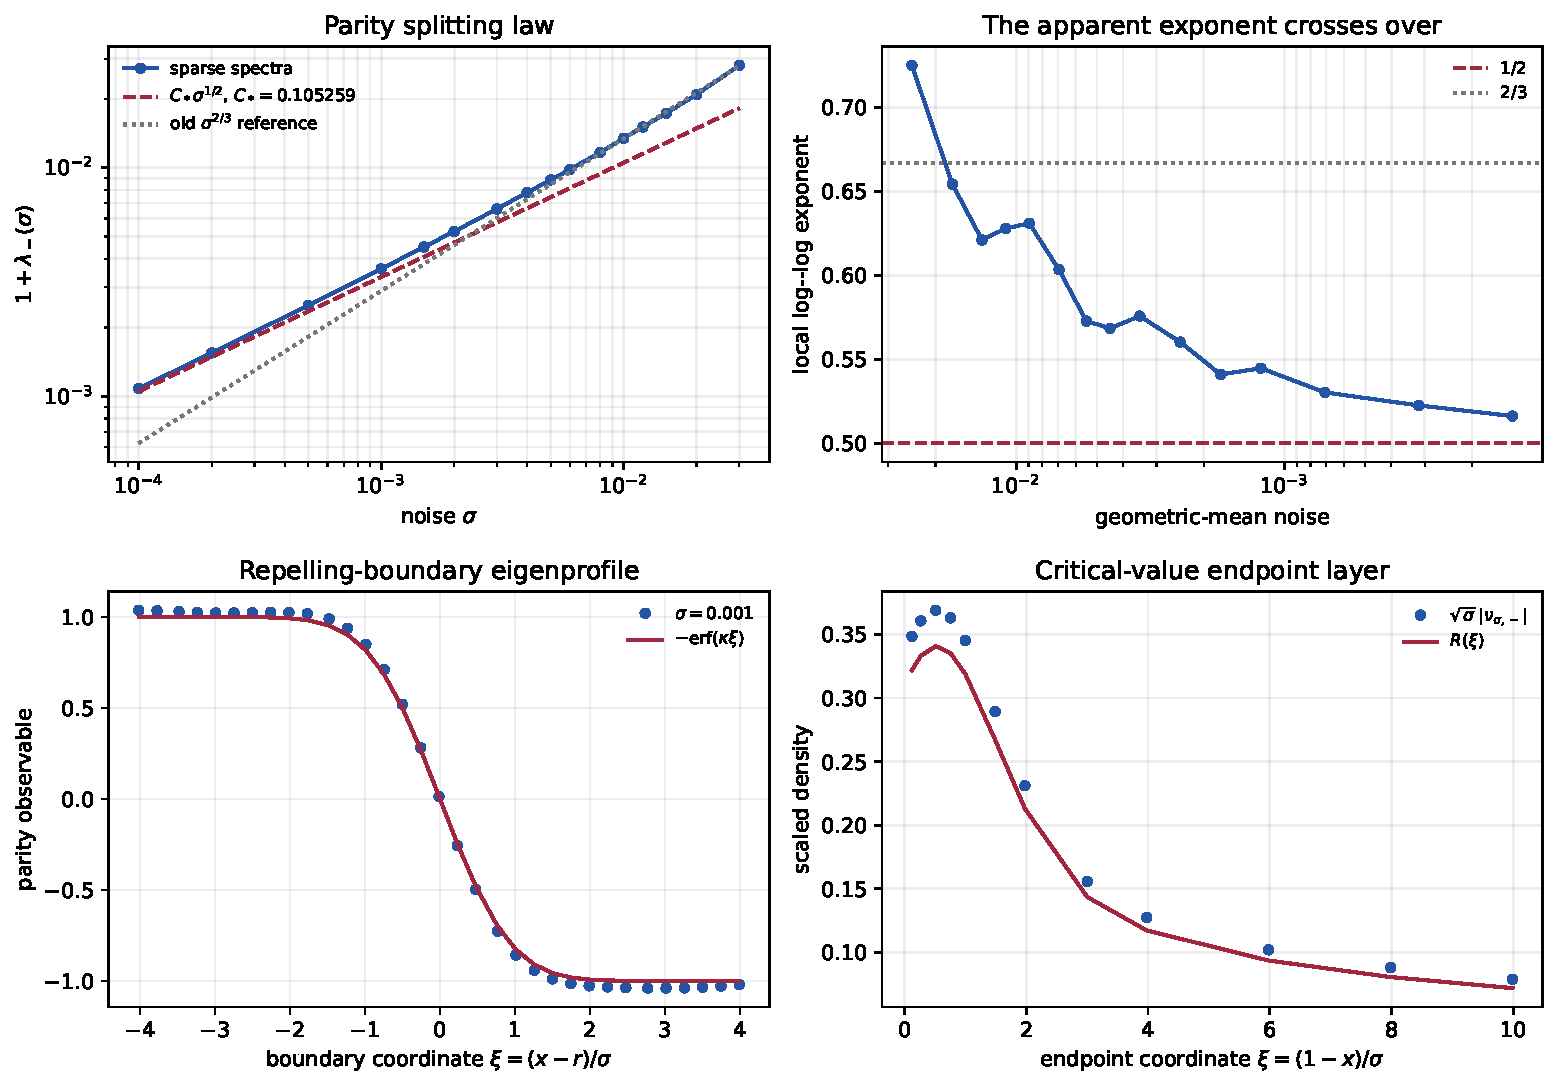
\includegraphics[width=\textwidth]{figures/square_root_parity_boundary_layer.pdf}
\caption{Square-root boundary-layer audit.  Top left: the extended parity
gap and the analytic square-root law; the dotted $2/3$ reference only follows
the intermediate window.  Top right: local exponents drift from the old fit
toward $1/2$.  Bottom left: the right matrix eigenvector collapses onto the
exact error-function boundary profile.  Bottom right: the left signed
eigenvector density approaches the independently derived critical-value
profile $R$.}
\label{fig:boundary-layer}
\end{figure}

\subsection{Resolution and profile checks}

At $\sigma=0.001$, increasing $d\sigma$ from $10.24$ to $30.72$ changes the
negative eigenvalue by only $6.40\times10^{-6}$, or $0.18\%$ of the parity
gap.  The value at $d\sigma=20.48$ differs from the finest one by
$9.98\times10^{-7}$.

The lower panels of \cref{fig:boundary-layer} test the two ingredients of the
proof separately at $\sigma=0.001$, $d=20480$.  The observed parity
observable differs from $H$ by at most about $3.7\%$ on
$|\xi|\le4$.  The endpoint signed density has an $8$--$10\%$ preasymptotic
offset but follows the full shape of $R$, including its nonmonotone maximum.
Neither profile is fitted to the matrix data: $\kappa$, $a$, $\rho_c$, and the
row-normalization factor are fixed before diagonalization.

\begin{figure}[H]
\centering
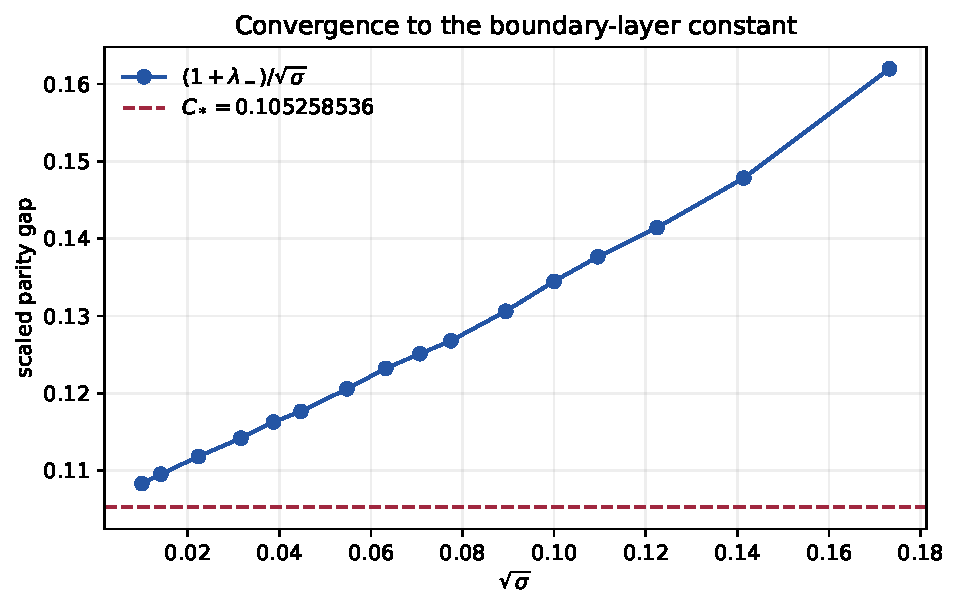
\includegraphics[width=0.76\textwidth]{figures/square_root_constant_convergence.pdf}
\caption{The scaled gap $(1+\lambda_-)/\sqrt\sigma$ approaches the
boundary-layer constant $C_*$.  The horizontal value comes from
\eqref{eq:C-double}, not from regression against the resonance data.}
\label{fig:constant}
\end{figure}

\subsection{Reproducibility and numerical status}

The sparse calculation at $\sigma=10^{-4}$ has $204800$ states and
$6.77\times10^7$ nonzeros.  The archived output contains all sixteen noise
levels, five independent resolutions, both profile tables, software versions,
and source hashes.  The test suite checks the sparse/dense spectral match, the
Taylor stability of $\rho_c$, the exact Gaussian eigenprofile identity, the
nested integral for $C_*$, and a finite-noise parity resonance.

The quadrature and matrix eigenvalues are ordinary floating-point
computations.  They support the displayed decimals and figures but are not a
computer-assisted proof.  The theorem asserts an exact positive integral
constant and the exponent $1/2$; neither assertion depends on a rounded
eigenvalue or fitted slope.

\section{Discussion}
\label{sec:discussion}

\subsection{Why the exponent is one half}

The critical source scale is $x=O(\sqrt\sigma)$ because
$1-f(x)=\uc x^2$.  It creates an endpoint density of height
$\sigma^{-1/2}$ over a layer of width $\sigma$.  The endpoint then maps to
the parity boundary, where the error-function profile has an $O(1)$
solvability defect.  Thus
\begin{equation}\label{eq:dimensional-balance}
 \underbrace{\sigma^{-1/2}}_{\text{critical density}}
 \times
 \underbrace{\sigma}_{\text{endpoint width}}
 \times
 \underbrace{1}_{\text{parity defect}}
 =\sqrt\sigma.
\end{equation}
The exponent is therefore geometric, not a free regression parameter.

The repelling boundary $r$ is essential but does not itself generate the
splitting.  Its local Gaussian dilation problem is exactly solvable at
eigenvalue $-1$.  The gap appears because the second preimage $x=1$ ends at
the state boundary and is fed by a quadratic critical point.  This is why a
one-layer leakage estimate misses both the constant and, over moderate noise,
the apparent exponent.

\subsection{The corrected two-clock picture}

The deterministic periodic-orbit localization method has the logarithmic
ceiling
\begin{equation}\label{eq:log-clock}
 m_{\mathrm{loc}}(\sigma)
 \lesssim\frac{\log(1/\sigma)}{\log\lambda}
\end{equation}
because some cycles approach the state boundary exponentially
\citep{WangLongCycle2026}.  The parity lifetime is now
\begin{equation}\label{eq:sqrt-clock}
 m_{\mathrm{par}}(\sigma)
 \sim C_*^{-1}\sigma^{-1/2}.
\end{equation}
It remains parametrically longer than \eqref{eq:log-clock}, although shorter
than the previously conjectured $\sigma^{-2/3}$ scale.  At
$\sigma=10^{-4}$, the resolved e-folding time is about $923$, while the
leading formula gives $950$ and the logarithmic orbit ceiling is only about
$17.8$.

This separation is constructive.  It says that a simultaneous
small-noise/long-cycle determinant cannot be obtained by extending isolated
periodic Gaussian tubes to the parity lifetime.  The correct intermediate
description must first extract the factor
$1-z\lambda_-(\sigma)$ and treat the two coupled boundary layers before
attempting a bulk determinant limit.

\section{Conclusion}

The noisy parity resonance at the quadratic band-merging parameter has a
nonanalytic but explicit small-noise splitting.  The component-boundary
observable is an exact error function, the critical endpoint density is a
normalized Gaussian--quadratic integral, and their solvability pairing gives
\[
 1+\lambda_-(\sigma)
 =0.105258535936908\ldots\sqrt\sigma+o(\sqrt\sigma).
\]
The formerly observed $2/3$ exponent is a genuine and reproducible
intermediate-window fit, but it is not the asymptotic law.

This closes the stochastic parity question left by the long-cycle analysis:
the negative resonance converges to $-1$, its lifetime scale is
$\sigma^{-1/2}$, and the crossover profile is explicit.  The next spectral
gate is no longer an exponent fit.  It is to determine whether the
parity-extracted noisy bulk determinant has a target-independent scaling or
scattering limit.

\section*{Data and code availability}

The source, tests, sparse spectra, resolution audit, boundary profiles,
figures, and machine-readable summary are archived with this paper
\citep{WangBoundaryLayerCode2026}.

\bibliographystyle{plainnat}
\bibliography{references}

\end{document}
